\documentclass[conference]{IEEEtran}
\IEEEoverridecommandlockouts
% The preceding line is only needed to identify funding in the first footnote. If that is unneeded, please comment it out.
\usepackage{cite}
\usepackage{amsmath,amssymb,amsfonts}
\usepackage{algorithmic}
\usepackage{graphicx}
\usepackage{subfig}
\usepackage{textcomp}
\usepackage{xcolor}
\def\BibTeX{{\rm B\kern-.05em{\sc i\kern-.025em b}\kern-.08em
    T\kern-.1667em\lower.7ex\hbox{E}\kern-.125emX}}    
\usepackage{makecell,rotating}
    \setcellgapes{5pt}
\pagestyle{plain}   

    
\begin{document}

\title{Methods for Wide Area Network Capacity Planning for Internet Services\\
%{\footnotesize \textsuperscript{*}Note: Sub-titles are not captured in Xplore and
%should not be used}
%\thanks{Identify applicable funding agency here. If none, delete this.}
}

\author{\IEEEauthorblockN{Eric Kumar}
\IEEEauthorblockA{\textit{School of Architecture} \\
\textit{Carnegie Mellon University}\\
Pittsburgh, PA USA \\
ekumar@andrew.cmu.edu}
}

\maketitle

\begin{abstract}
This paper reviews internet scale applications that are driving near exponential growth of wide area networks (WAN) for data-centers. The methodology takes page level user requests and converts them to network link demand in bits using minimum distance functions and several layers of aggregation.  Three years of time series data is split into training and testing sets for forecasting and validation. Forecasts are done with two methods, namely ARIMA and Facebook's Prophet. The power capacity of respective data-centers is used to allocate workloads. A method for event based changes to the network flows is also presented. This work finds that the Prophet model is superior to ARIMA to forecast web-traffic. 


\end{abstract}

\begin{IEEEkeywords}
wide area network provisioning, replication, backbone networks, network capacity
\end{IEEEkeywords}

\section{Executive Summary}

Users of web services demand high availability of data in diverse sets of operational environments. Web services respond with databases that provide strongly consistent data for users regardless of their location. High availability targets drive online platforms with distributed database architecture to also be agnostic to component level failures. In these environments component failures are random and exponentially correlated with the scale of the systems. Compounding the equipment failures is the vulnerability presented when a network link is partitioned, preventing communication between fully functional nodes. 

Despite the need, it has been proven that Consistency, Availability, and Partition tolerance (CAP) can not co-exist against in distributed systems by the CAP Theorem \cite{CAP}. However, proper network planning with sufficient capacity and multi-path redundancy do mitigate the risk of network unavailability and minimize the chances of partitioning (cutting a link).

WANs are not just a diaster recovery mechanism. Strategic provisioning of WAN lifts the overall system performance as well. Reffering to Amdahl's law, which is based on that observation that when a process segment is sped up, the effect on the end to end process time is dependent on how significant the part originally was and the incremental speed gain. Table \ref{dean} lists the latency associated with different components in a distributed systems stack, \cite{Dean}. At global scale, improvements in network latency can contribute upto 10 factors of magnitude more significance to speed up the end to end process than L1 cache. It is also generally accepted that higher ranking components in the list have higher unit cost per bit of capacity \cite{Bryant}. Given the impact and cost per bit of network, this work aims to quantify the capacity ceiling which alleviates the WAN as constraining factor for distributed systems. Here the several long term planning methods that bin pack multiple communications flows are logically decoupled is explored. Logically decoupled flows, in this context, are service communications that share source and destination points yet their bandwidths are independent variables. In such cases, a collection of flows may have diverging patterns or may simultaneously converge as independent variables.
 
\begin{table}[htbp]
\caption{ Process Latency Scale, \cite{Dean}}
\begin{center}
\begin{tabular}{ll}
\hline
\textbf{Component} 					& \textbf{Latency} (ns)	\\
\hline
L1 cache reference					& 0.5					\\
Branch mispredict 					& 5					\\
L2 cache reference					& 7                     \\
Mutex lock/unlock					& 25					\\
Main memory reference				& 100					\\
Compress 1K bytes with Zippy 		& 3,000					\\
Send 2K bytes over 1 Gbps network	& 20,000				\\
Read 1 MB sequentially from memory	& 250,000				\\
Round trip within same datacenter	& 500,000				\\
Read 1 MB sequentially from disk	& 20,000,000			\\
Send packet from CA to Netherlands and back to CA 	& 150,000,000			\\
\hline
\end{tabular}
\label{dean}
\end{center}
\end{table}

Considering the CAP theorem and Amdahls law, service operators need to understand their networks. Operators need to sufficiently plan the size of the networks for normal and disaster recovery operations in the face of many failure modes of within the holistic system. This paper surveys several different data base systems and extracts their network dependency. It then evaluates three approaches to network planning based on traces obtained from Wikipedia.


\section{Introduction}

Web services are transactional and exhibit four key properties \cite{CAP}. (1) it is expected that transactions commit or fail across all instances instantaneously , (2) they always provide consistent data regardless of the location they are executed from, (3) uncommitted transactions are isolated, and (4) once committed they are persistent. For modern internet services, these properties and objectives are achieved with global scale data-replications strategies. The four service level properties are attributed to the three key design objectives listed below. 

\begin{itemize}
	\item Durability: Persistent in case of physical failures.
	\item Accessibility: Be able to use when needed.
	\item Performance: Get to it quickly.
\end{itemize}

Data-replication over the WAN facilitates redundant data to be cast into multiple nodes that are spread across geographically disparate locations. Disparately located redundant data allows a system to tolerate failure modes such as node outages or network partitions, making it an attractive choice when durability and availability of a system are design objectives. Replication strategies are also used to enhance performance of globally distributed internet services. First by allowing faster user access to data with minimum distance optimizations when serving requests. Secondly for distributing the read requests over more nodes and balancing the load on them. The former reduces communication latency and the latter reduces queing latency that would arise if all read requests were sent to a single node. However, when there are multiple copies of the same data there is a risk for them to not be consistent with each other due to communication latencies and failures in the system.

There are three methods for data-replication widely used today and each offers a different degree of trade-off between consistency and latency \cite{Abadi}. The first method has minimal latency where updates are multi-cast to all the replicas simultaneously. However, isolated clients (external consumers of the data-base) may send multiple updates that are received out of order due to communication delays leading to over-writes. The second scheme has updates routed to a designated master node which has the purest and most up-to date view of the data-base. The master node then replicates to all replicas either synchronously or asynchronously. The third scheme sends updates to an arbitrary node, which records that data and make to replicas and users with local access. One shortfall with this approach is upon failure of the arbitrary node, unrecorded and forwarded data maybe lost/

Given the dependence on replication for internet service and it's sensitivity to latency, it is crucial that WANs be properly provisioned with sufficient capacity and redundancy in order to negate congestion that leads to delays. In the motivational work section, several modern data-base systems and their replication strategies are reviewed. The review finds that the published DB system present an abstracted view of their network dependency. Therefore physical implementation of the network architecture may be proprietary and distinct from each other. To generalize the distinct implementations, the Background section first a develops a hierarchical clos topology to provide intuition about the rest of the paper. The Methodology section presents several approaches to estimating bandwidth requirements. These methodologies are then evaluated and compared to each other for a typical uses case in the results sections. This paper concludes with the Conclusion section. For brevity, this work only considers a single class of network traffic. 

\section{Motivational Applications}

Wide area networks serve as the backbone for many internet applications that operate across regional data-centers. The traffic on the inter data center links are segregated into three classes; interactive, large file transfers, and background \cite{Zhang}. Interactive traffic are blocking operations; where the byte level transactions are required to keep things proceeding. Large file transfers entail transmission of requested resources by some deadline. Background traffic are workloads that are opportunistically using the link, and preempting them does not expose the system of any idempotent side effects. DB communications traffic typically consists of workloads that are bound by deadlines and also pseudo-interactive. This section presents a sample of specific database system that serve as back-ends for many modern online platform architectures. 

%MS-SD WAN

Megastore was the first large-scale system to use Paxos to replicate primary user data across regionally distributed data-centers for every write \cite{megastore}. Megastore enables applications to have fine grained control for partitioning and locality by Entity Groups. Several entity groups in Megastore are provisioned across a set of data-centers. Locally, the distinct entity groups have loose consistency requirements however common entity groups across data-centers maintain atomic, consistent, isolated, durable (ACID) data over the WAN. Megastore relies on the underlying Bigtable \cite{bigtable} instances at each of Google's data-centers. Megastore implements a multiple version concurrency control schema, that allows DB fields to have multiple versions isolated by time-stamps. This eliminates interference between reads and writes, as reads will be fetched from the most completed time-stamp DB. Megastores has several types of logical actors. Namely they are leader, full-replicas, witness, read-only. Witness actors vote in Paxos rounds and store write ahead logs, but are thrift on storage for entities. Read only actors provide present views of the data based on a near real time snapshot.

Spanner is a gloablly distributed database in which writes are committed with the Paxos protocol at single leader node. Reads access the data directly from any replica  that  is  sufficiently  up-to-date, which can have service garantees in terms of consistency classes.  The  set  of replicas is collectively a Paxos group \cite{Spanner}. As a globally distributed database, Spanner provides several interesting features, \cite{Spanner}. These features faclitate replication configurations to be dynamically controlled at by applications with . First, applications can specify constraints to control which data centers contain which data. Second, it allows application owners to specify how far data is from its users (to control read latency). Third, application owners to delegate how far replicas  are  from  each  other  (to  control  write  latency). Finally, applications can control  how  many  replicas  are maintained (to control durability, availability, and read performance). 

In the Google Cloud Platform Console, the most economical multi-region Spanner instance, nam3, notes the following specs. Nam3 consists of 3-way redundancy with-in North America. It provides an availability service level objective (SLO) target of 99.99\%. In contrast to a single region Spanner instance which yields a 99.9\% SLO. 


\textbf{Spanner Guidelines}
\begin{itemize}
 \item Each Cloud Spanner node in nam3 can provide up to 7,000 QPS (queries per second) per region, or 1,800 QPS of writes across all regions for writing 1 kB data per row with total storage capacity of 2TiB.
 \item For optimal performance in this configuration, it is recommended that CPU utilization be maintained at at or below 45\%.
 \item A minimum of 3 nodes is recommended for production environments; ie user facing.
 \item Cloud Spanner's performance is highly dependent on workloads, SQL schema design, and data-set characteristics. 
\end{itemize}

Cassandra is a NoSQL database open sourced by Facebook \cite{Cassandra}. Cassandra's architecture is based on a coordinator paradigm, where the consistency level is user defined and a coordinator node is responsible for forks and joins of the data to yield either a single view, quorum view ($(\frac{Nodes}{2} +1)$), or all views of the data. Each node in the Cassandra architecture is configured to directly communicate with clients. To illustrate, clients reading some data connect with a single Cassandra node. Upon receiving the request, the Cassandra node presumes the coordinator responsibility and retrieves data from its local storage and/or coordinates its retrieval based on the consistency level required by the request.

MongoDB Atlas is a open sourced MongoDB NoSQL database offered on the cloud \cite{Mongo}. Cloud distributed Atlas consists of a set of upto 50 replicas with one primary replica member and the balance serve in secondary replica member roles. Upon a failure of the primary, one of the secondary members is automatically upgraded to primary based on an election process. The promotion of a secondary node to primary takes on the order of a few seconds, at which point clients direct their connection to the new primary for writes. Reads are still facilitated at all available nodes without disruption. Atlas' primary election process is implemented with the Raft consensus protocol \cite{raft}. First, the protocol evaluates replica based on their state, biasing towards replicas that have the most recent updates applied. Second, Atlas' RAFT checks the heartbeat and connectivity status of a quorum of replica set members. Finally, the algorithm allows administrator to configure a deterministic preference of the replica set to promote. With a replicas promoted all secondary replicas redirect their connection to it. 

In MongoDB Atlas data is horizontally spread across physical servers by using sharding techniques. Sharding of values in a data set can be done locally with-in a single data-center, or distributed globally across the replica-sets. Each shard has a replica set consisting of primary and secondary members as shown in \ref{mongo_shards}. The shards are made transparent to clients with the use of local "Query Routes" as an abstraction layer. When reading, the default is to read from the primary member but users can set reads to be from the nearest replicas for minimum latency at the cost of consistency. Writes can be acknowledged from the primary only, a deterministic count of replicas, the quorum of replicas, or all replicas. There is an option for completely unacknowledged writes. To relieve the burden on the network demand, application layer data is compressed upto 80\% for transport across the network. Users can specify weight for writes to specific data-centers and apply higher relative weights to Primary DC's.

\begin{figure}[htbp]
\centering
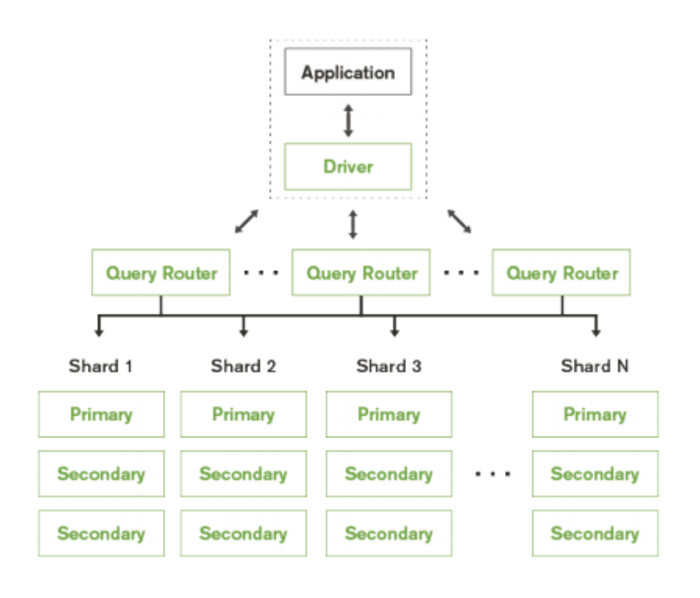
\includegraphics[scale=.5]{mongo_shards.eps}
\caption{MongoDB Atlas Sharding Scheme \cite{Mongo}}
\label{mongo_shards}
\end{figure}

To appreciate the complexity of distributed systems quantitatively, the Storage Configuration Compiler (SCC) provides a broadview of the interaction between various componets of a distributed storage system \cite{scc}. The Storage Configuration Compiler is a tool that takes an application's service level objectives, storage hardware parameters, and compute server parameters along with their costs to suggest optimum cluster configurations. At the application level SCC separates tasks and data sets. Data-set accessibility is treated as a non-deterministic variable and each operation is modeled as a probability function. It is shown explicitly in SCC that network delays hang-up machine resources waiting for responses, wasting expensive resources. 

\textbf{Storage I/O throughput definitions for SCC:}
 \begin{itemize}
 \item read/write gap parameter for non-sequential seeks.
 \item $\frac{size}{rate}$ + gap is the latency to serve 
 \end{itemize}

\textbf{I/O operations definition for SCC:}
 \begin{itemize}
 \item Number of records read in an I/O operation
 \item Number of records written in an I/O operation
 \item Bytes count of each record
 \item Are the reads parallel
 \end{itemize}

\textbf{Task Dependencies:}
\begin{itemize}
\item The count of invocations being performed
\item are the invocations in parallel
\item is the whole dependency block or non-blocking
\end{itemize}

\textbf{Capacity Parameters:}
\begin{itemize}
\item data set size
\item does it need to be persistent
\item local or remote
\end{itemize}


\section{Background}
This section provides context about the current industry trends. The next paragraph argues that local costs optimization increases the reliability burden for global presence. The following subsection then presents the bounds of data communication networks is presented from the data-center level to the wide area networks that connect  data centers. 

The current data center market has two paradigms for cost savings, one is hardware based and another infrastrucutre based. The hardware based paradgim consists of the mentatlity that more of cheaper hardware are better than less of expensive ones. Parrallelsim is increased with more hardware node counts leading to faster end to end processes, compared to using few high cost machines yeild a performance/\$ efficiency gains. More hardware counts do allow more local redundanency. Replication at locally housed servers increases data availability in the presence of individual server failures, but only with diminishing returns \cite{megastore}. 

The infrastructure costs savings are based on relaxing tried and trued industrial practices, examples being free air cooling that introduces contamination or removing UPSes from the power delivery systems. The utility scale systems such as power, cooling, and long haul tele-communication networks introduce additional risk that is not offset by local replication. It has been pointed out that hyperscale internet data-centers are susceptible to construction value engineering that risk some level of facility-wide failure modes \cite{wsc}.

\subsection{Context Setting}

To motivate interest in the rest of this paper, let's visit some typical conisderations that are encountered in industry. First, applications need to understand their distributed process latencies. In the absense of network congestion, the ideal elapsed time ($t_e$) to transfer B, bytes, to R, replicas, is shown in equation \ref{replication_time}. $T$ is the network throughput rate in bytes per unit of time and $L$ is latency to transfer bytes between two machines\cite{GFS}. Network links are typically on the order of \textit{O}(xx)-Gbps (T), and $L$ is far below 1 ms as seen for component level contributions in Table \ref{dean}. Therefore, 1 MB can ideally be distributed in about 80 ms. As a contextual example, an average text heavy Wikipedia article is about 5.2 MB.

\begin{equation}
\label{replication_time}
t_e = B/T+RL
\end{equation}

Second, applications need to understand the statistical distribution of their communication capacities. To demonstrate this, it is most intuitive to consider a local data-center environment as seen by a server on a rack. Maximum bandwidth that a server can send out of a rack is limited by the top of rack (TOR) outbound channels. As an example, if a rack consists of 35 servers, each connected to the TOR at 10 Gbps channels. With a TOR capacity of 100 Gbps to its external adjacencies, only 10 of the servers can sustain full bandwidth.  Equation \ref{TOR} indicates the limit of the flows from all servers in a rack must be equal to or less than the TOR's external facing capacity. However, servers with-in a rack can also communicate with each other and not be limited by the TOR's external limits. An depiction of the complete topology is shown in \ref{DCN}.

\begin{figure}[htbp]
\centering
\includegraphics[scale=.35]{rack_view.png}
\caption{Request Ingress and Responses from rack perspective.}
\label{DCN}
\end{figure}

\begin{equation}
\label{TOR}
TOR \geq \sum{I_{i}}
\end{equation}

\begin{footnotesize}
Where: \\
\indent TOR: Rack level ingress and egress bandwidth to external adjacency.\\
\indent $I_{i}$: Server level ingress and egress network bandwidth.\\
\end{footnotesize}

The schematics of over subscription can be found throughout the network stack, spanning from the chip scale components to global scale networks. In case of demand exceeding the capacity of the blocking upper hierarchy, packets are either lost or are buffered in a queue. Some popular cloud WAN networks are reducing their queue sizes for WANs. In these cases at times of congestion more in-transit packets are simply dropped and the pending packets in the TCP ports are held locally at the clients until congestion disappears \ref{B4}. This puts more burden on the network as packets will need to be re-transmitted, lowering the percentage of good put on the links due to multiple transmissions of the same packet. This also has impacts on the servers and storage workloads, as the will need additional capacity to fetch the data or run the task gain. 


\section{Methodologies}

In this section three forecasting methods are discussed. The methods are time series projections, event based projections, and power based based projections. Wikipedia page view data is used to demonstrate the application of each method presented. The approach described in this section resemble those used by aggregate network planners, where numerous independent services are bin packed into a network flow from a source node to a destination node.  

The time series method in this work first establishes a benchmark with the data-set discussed below. Benchmarks that correlate to other resource dimensions provides more robust signals for network capacity demands earlier. In a simple example, workers (computers) are required to generate network traffic. Without specific computer resource knowledge, the traffic to each ingress site is considered the system's demand. The time series ingress site load profiles provide the benchmark to size network links from them to the primary data-center.  

In Cloud enviroments agility is also a key criterion \cite{Spanner}. First agility is needed when new users and services are on-boarded. Secondly, new features that increase network efficiency or new use cases of network are continuously added. Finally, the decoupling of physical resources from logical resources have enabled container type, elastic workloads. The containers not only dynamically change resource dimensions but can also physically migrate across the globe without much effort. These use-cases necessitates event based models. 

Power based load profiles are the most coarse form of modeling network demands. However, power maybe the only known variable at the lead times for network links that maybe 1.5 to 5 years out. For example, many data-center builders do not know the tenants or services that will be housed within their facilities when they design and build their sites. The problem is prevalent for large private operators who own and run their data centers for internet services and technologies that iterate much faster than network link lead times. This problem is compounded for colocation or Cloud data-center owners who have little influence on their occupants network demands.

The three approaches explored in this work are sufficient to forecast IP network traffic in the leads times that operators are bound to. Specifically the data-set chosen allows all three methods to be developed in the context of real world internet traffic profiles. Another important aspect of Wikimedia's data-set is that it is non-proprietary, while still showing the complexities of modern internet loads at a global scale.

\subsection{Data Set}
Traffic to 145,063 Wikipedia Pages for 803 days from July 2015 through September 2017 is used demonstrate the scale of replication required for global services. The data will be used to train and test the models developed here. The training set will be partitioned to be inclusive of traffic from July 2015 to December 2016. The balance of the data will be used to test accuracy of the models. The pages are segregated into 7 different languages; namely English, Japanese, German, French, Chinese, Russian, and Spanish. The average volume of visits per language is shown in Figure \ref{average_use}. Figure \ref{95_tile} shows the distribution of the 95 percentile usage values per respective language.


\begin{figure}[!tbh]
  \subfloat[Average]{\includegraphics[width=0.25\textwidth]{average_use.jpg}\label{average_use}}
  \subfloat[95 percentile]{\includegraphics[width=0.25\textwidth]{quantile95_use.jpg}\label{95_tile}}
  \caption{Visits to Study Set of Pages by Language}
\end{figure}

After segregation of the pages by language and dropping pages without language indicators, the languages are mapped to countries in which they are the official tongue. Figure \ref{world} shows the mapping of languages to their respective countries by color groups; English(blue), Japanese(dark gray), German(yellow), French(red), Chinese(green), Russian(orange), and Spanish(magenta). Red markers indicate the locations of Wikipedia data centers from around the world as listed in Table \ref{wiki_dc}. Ashburn has the primary (P) data-center for application services, and Carrollton serves as the redundant (R) node. The remaining 3 sites are smaller edges of the Wikipedia network where user traffic ingresses and egresses Wikipedia network. 

Throughout this paper the associated set of Wikipedia data-centers is used to model its network and several assumptions are called out in regards to attributes of the system that are not in the public domain. Furthermore, some of the system complexity is reduced for brevity and academic objectives of this work. The traffic generating in a particular country is associated with their closest ingress points as listed in Table \ref{ingress_lang} by using a minimum distance function between respective geographical coordinates. This table shows that English is the most dominant language with traces appearing at all of Wikipedia's ingress sites, with originating from 49 countries.

\begin{figure}[htbp]
\centering
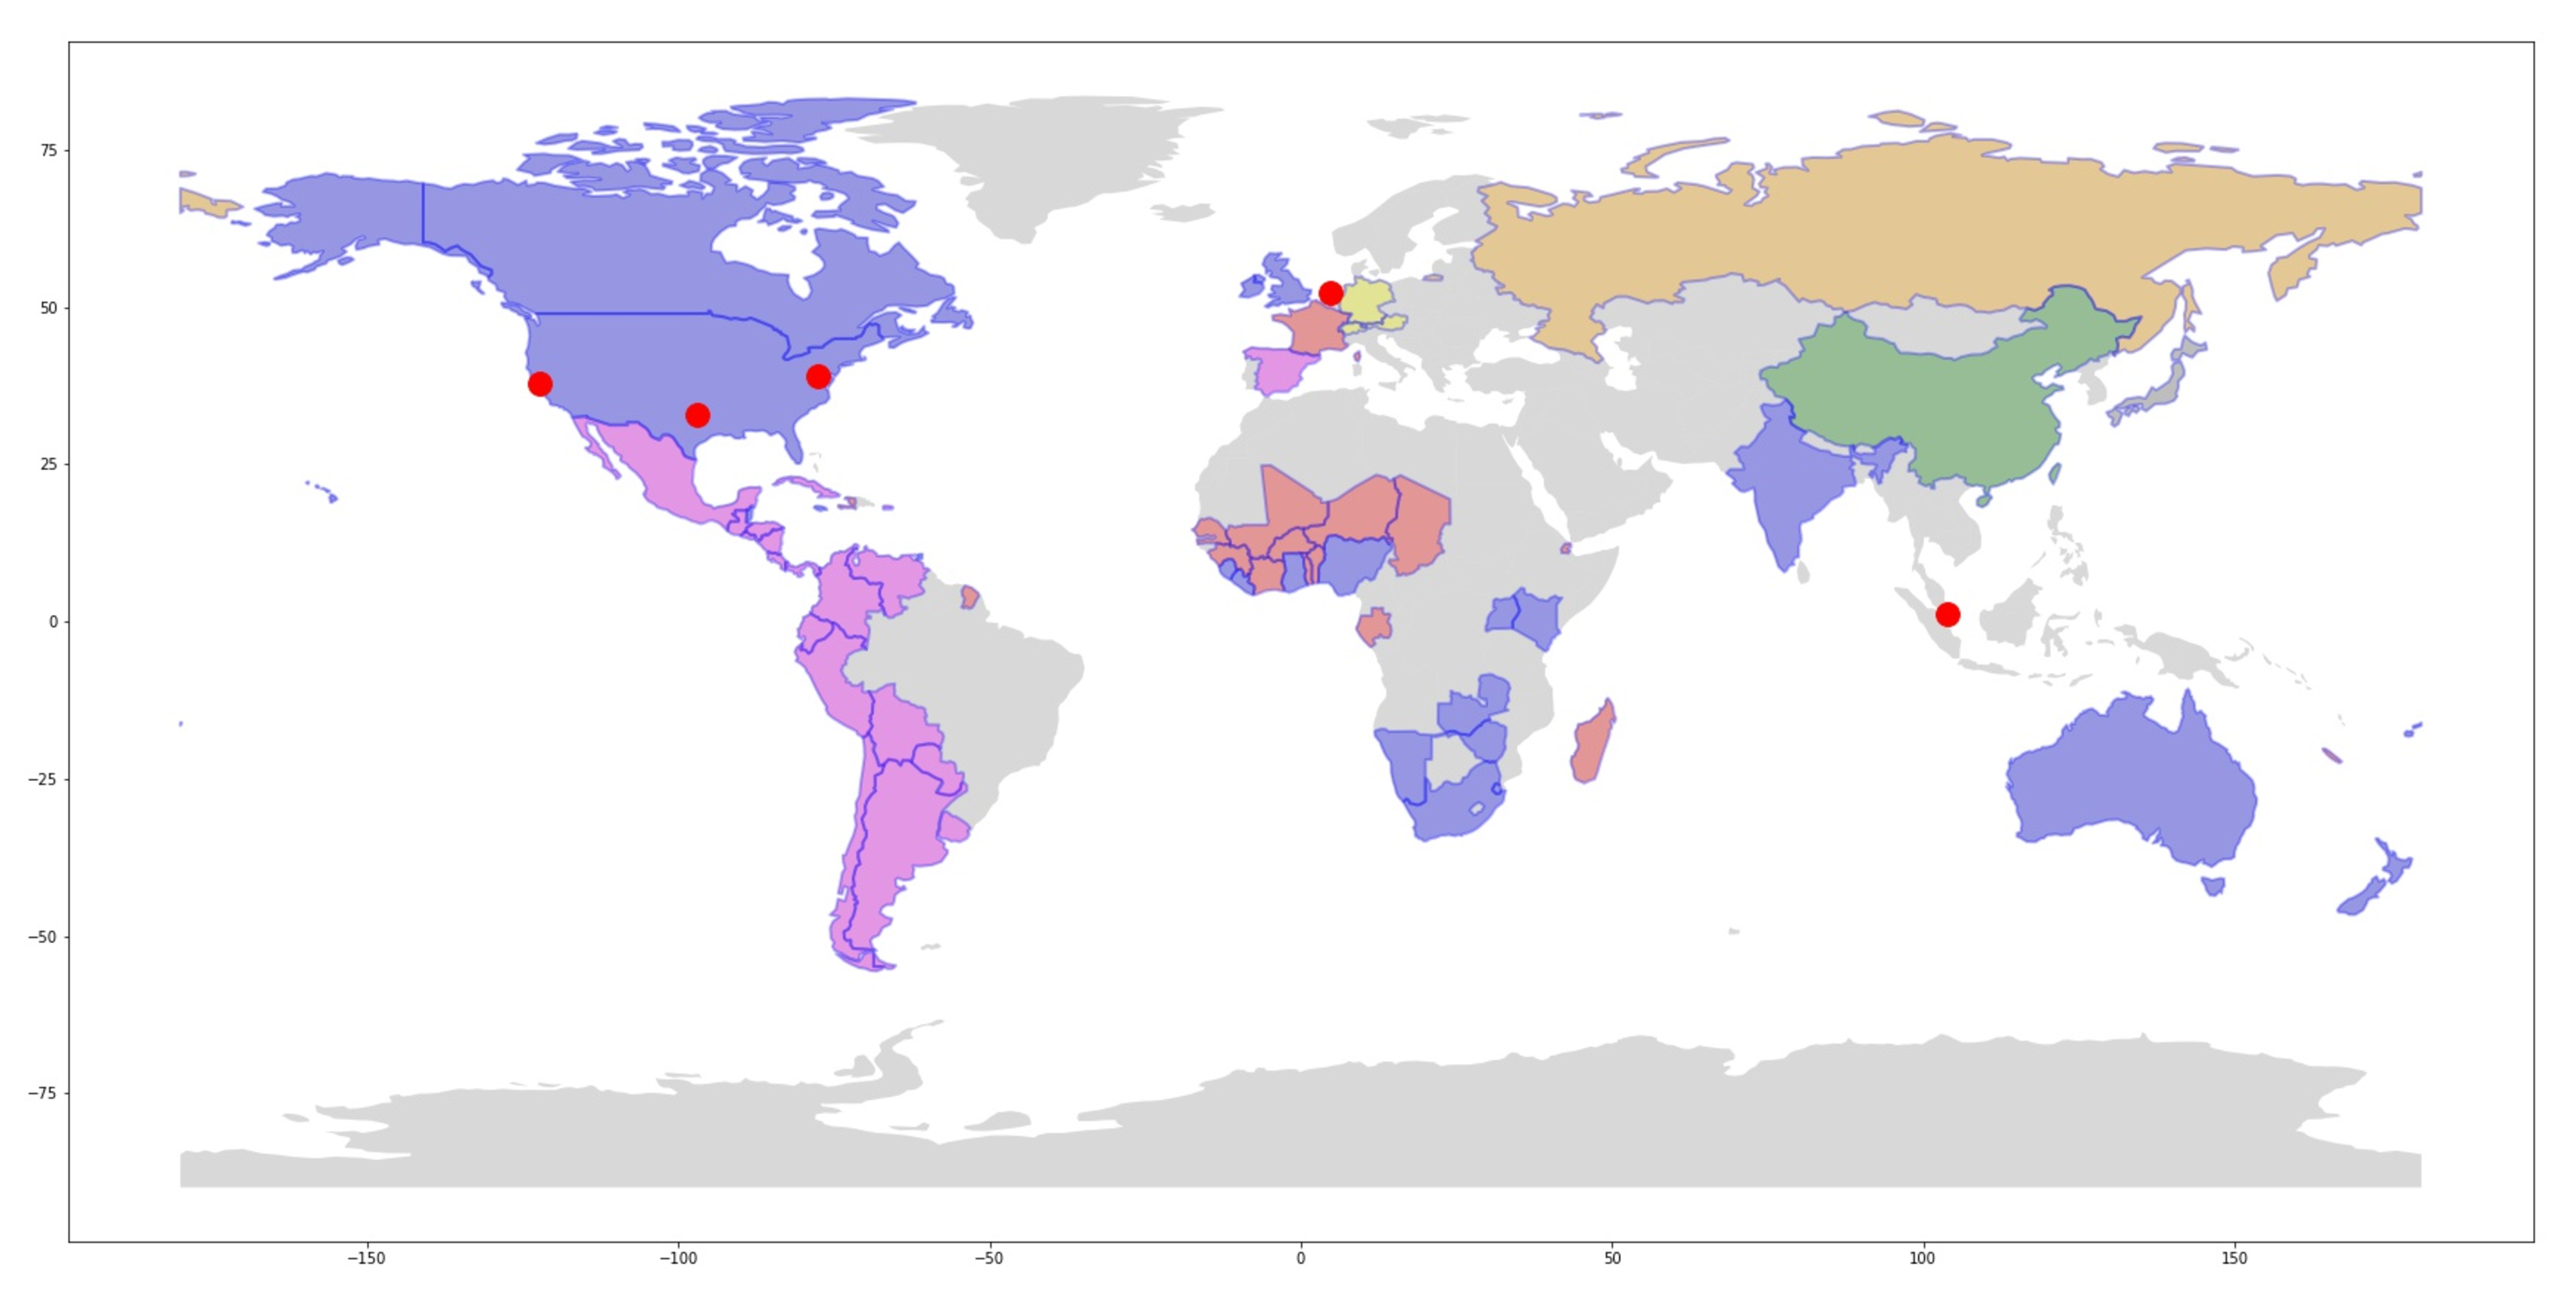
\includegraphics[scale=.15] {world.eps}
\caption{Countries of origin for traffic by language}
\label{world}
\end{figure}

\begin{table}[htbp]
\caption{Wikipedia Network Nodes}
\begin{center}
	\begin{tabular}{|c|c|c|c|c|}
		\hline
	{} &         ID &  Address                  & Power(kW) & Type \\
		\hline
	1 &       eqiad &  Ashburn, Virginia, USA   & 130-kW    & Applications-P \\
	2 &       codfw &  Carrollton, Texas, USA   & 77-kW     & Applications-R  \\
	3 &       esams &  Haarlem, Netherlands     & $<10$-kW  & Caching  \\
	4 &       ulsfo &  San Francisco, CA, USA   & $<5$-kW   & Caching  \\
	5 &       eqsin &  Singapore                & 10-kW     & Caching \\
	6 &       eqord &  Chicago                  & -         & Transit \\
	7 &       eqdfw &  Dallas                   & -         & Transit \\
	8 &       knams &  Amsterdam                & -         & Transit \\
		\hline
\end{tabular}
\label{wiki_dc}

\end{center}
\end{table} 

%this table is about 2 weeks of work
\begin{table}[htbp]
\caption{Languages to Ingress Sites}
\begin{center}
\begin{tabular}{|c|c|c|c|c|c|c|c|c|}
\hline
DC            &  en & ja & de &  fr & zh & ru &  es & \textbf{total} \\
\hline
Ashburn       &  17 &  - &  - &   5 &  - &  - &   8 & \textbf{31} \\
Carrollton    &   3 &  - &  - &   - &  - &  - &  11 & \textbf{13} \\
Haarlem       &  17 &  - &  4 &  16 &  - &  - &   1 & \textbf{38} \\
San Francisco &   3 &  - &  - &   1 &  - &  - &   - & \textbf{4}  \\
Singapore     &   9 &  1 &  - &   4 &  5 &  1 &   - & \textbf{20} \\
\hline
\end{tabular}
\label{ingress_lang}
\end{center}
\end{table}

Now, turning the focus to another key attribute noted in Table \ref{wiki_dc}, power. Most of the power values are obtained directly from Wikipedia reports \cite{wiki_servers}. No power capacity values for 'eqsin' data-center was exposed by Wikipedia. Therefore the power demand for the Singapore data-center has been estimated by doing a qualitative similarity analysis based on ingress traffic.

The time-series plot of the hit rate at each of the ingress data-centers results in Figure \ref{ingress_hitrate}. Singapore's average page views per day visually appears to dominate other data-centers for ingress traffic, yet it is a caching site so is only comparable to other caching sites. Haarlem generally tracks Singapore well, with only slight divergence during their peak traffic period. When quantified, the average hit rate of Singapore is 3\% higher than Haarlem. The traffic allocation approach is indicated in Table \ref{lang2bits}. Given the conditional $<10kW$ value provided by Wikipedia for Haarlem, Singapore is also determined to have a $10kW$ demand. 


\begin{table}[htbp]
\caption{Method for Traffic Allocation to each ingress site}
\begin{center}
\begin{tabular}{cl}
Objective: & Determine the hit rate of each ingress site.                 \\
\hline 
Step 1:    & Map language to page.                                        \\
Step 2:    & Map languages to countries where they are the first tongue.  \\
Step 3:    & Map ingress sites to countries with minimum distance         \\
           & function.                                                    \\
Step 4:    & Get distribution of  number of countries served by each      \\
           & ingress site.                                                \\
Step 5:    & For each ingress site, sum up the daily views of pages by    \\
           & the language. Multiply to relative fraction from step 4 -    \\
           & origin countries  with language to site / total number of    \\
           & (Count countries with language).                             \\  
         

\end{tabular}
\label{lang2bits}
\end{center}
\end{table}

\begin{figure}[!tbh]
  \subfloat[Page View Count]{\includegraphics[width=0.25\textwidth]{ingress_hitrate.jpg}\label{singapore}}
  \subfloat[Bit Count]{\includegraphics[width=0.25\textwidth]{ingress_95bits.jpg}\label{san_francisco}} 
  \caption{Workload at each site. a) the count of pages viewed. b) Bits of network demand for link from Ashburn .}
\end{figure}

In Table \ref{wiki_dc} there are three transit sites in the Wikipedia network also. These are considered as passive network nodes, in that no processing or storage is facilitated at the sites. Figure \ref{wiki_net} illustrates Wikimedia's autonomous network system. The nodes are per Table \ref{wiki_dc} and the colored lines indicate discrete network connections, annotated with their carrier and the latency. The adjacency matrix of source and destination locations as vertices is shown in Table \ref{adajacency_matrix}

By examination of Figure \ref{wiki_net}, there are several physical paths that connect the spoke or edge sites to each other. Where multi-path routing is possible, all links that are expected to be used in normal conditions must be scaled. The path may pass through equipment at other nodes complicating the overall complexity of system topology design. Complications such as over-subscription and the blast radius of failure modes increase for shared resources. This work does not account of multi-path allocation of physical capacity.

The data-set does not provide an explicit flag indicating read or writes. In this work, all of the access tasks listed  are considered to be reads. Writes are comparatively in low volumes \cite{wiki_stats2}. As such only reads are considered in this the scope of this work, but the methodology can be extended to include writes.


\begin{figure}[htbp]
\centering
\includegraphics[scale=.2]{wiki_net.png}
\caption{Wikimedia's AS14907 Network. Source \cite{wiki_network}}
\label{wiki_net}
\end{figure}

\begin{table}[htbp]
\caption{DC Adjacency Matrix}
\begin{center}
\begin{tabular}{p{1cm}|p{0.3cm}|p{0.3cm}|p{0.3cm}|p{0.3cm}|p{0.3cm}|p{0.3cm}|p{0.3cm}|p{0.3cm}}
{}    & \rothead[c]{EQIAD}& \rothead[c]{ESAMS} & \rothead[c]{EQORD} & \rothead[c]{KNAMS} & \rothead[c]{CODFW} & \rothead[c]{ULSF} & \rothead[c]{EQSIN} & \rothead[c]{EQDFW} \\
\hline
EQIAD &     - &     2 &     1 &     1 &     3 &     - &     - &     - \\ \hline
ESAMS &     2 &     - &     - &     1 &     - &     - &     - &     - \\ \hline
EQORD &     1 &     - &     - &     - &     1 &     1 &     - &     - \\ \hline
KNAMS &     1 &     1 &     - &     - &     - &     - &     - &     - \\ \hline
CODFW &     3 &     - &     1 &     - &     - &     1 &     1 &     1 \\ \hline
ULSFO &     - &     - &     1 &     - &     1 &     - &     1 &     1 \\ \hline
EQSIN &     - &     - &     - &     - &     1 &     1 &     - &     - \\ \hline
EQDFW &     - &     - &     - &     - &     1 &     1 &     - &     - \\ 

\end{tabular}
\label{adajacency_matrix}
\end{center}
\end{table}

The network demand is derived from the ingress profiles at each site. Since the ingress sites only have a sub-set of their data cached locally, they require connections to the Ashburn site to retrieve additional data. Therefore, four links must be provisioned at sufficient capacity for the retrieval tasks by the remote ingress nodes; namely the node pairs connected by the links are (San Francisco, Ashburn), (Carollton, Ashburn), (Haarlem, Ashburn), and (Singapore, Ashburn). The cache hit-rate, that is the probability of requested data being locally available is determined on a relative power basis for each site as a ratio of the ingress site's power and the replica power capacity in Carrollton. The replica size in Carrollton is a discounted by 10kW as it alss serves as an ingress point. The Carrollton replica is chosen as Ashburn may support other processing and directly serve a significant portion of traffic.

\subsection{Power Allocation Method}

The power allocation method is inspired by the Gravity Model as proposed for capacity planning for telephony traffic between two area codes \cite{Gravity}. Strength of the interaction ($S$) between two area codes is proportional to the product of their populations ($P_g$) divided by the distance between them squared ($d$), see equation \ref{Gravity_city}. 

\begin{equation}
\label{Gravity_city}
S = \frac{P_g}{d^2}
\end{equation}

Data-center capacity is typically measured in terms of nominal power supported by the facility \cite{wsc}. As such, power capacity can be treated as being analogous to population for a data-center gravity model. For performance, power translates linearly to the computational capability of the system for a given set of hardware architecture. Here nominal power values are considered in a network flow directed graph, where the data-centers are the nodes (vertices) and the network communication link between two nodes are edges (arcs) of the graph. The rest of this section describes a power allocation method for establishing node and edge weights.

Consider the network of Wikipedia data-centers listed in Table \ref{wiki_dc}. The caching sites consists of front-end services, they only store fresh or the most popular copies of data for the local user base (see Figure \ref{world} and Table \ref{ingress_lang}). The data is presumed to be read only at the cache sites, and all writes are done in the primary application site. 

The average power use for each of Wikipedia's data-centers is shown in Table \ref{power_dist}. The power sums to 232-kW for all the data-centers by Equation \ref{eq:total_power}. Notice that EQIAD constitutes 56\% of the total power since all data is processed there by equation \ref{eq:percentage}. This is meaningful for network topology in that all data not cached locally at the ingress data-centers are sourced there, and for this topology Ashburn is always the source location. This drives the demand for sufficient bandwidth between EQIAD and all other sites for reads. .

\begin{equation}
P_{T}=\sum{P_{dc_i}}\label{eq:total_power}
\end{equation}

\begin{equation}
p_{dc_i}=\frac{P_{dc_i}}{\sum{P_{dc_i}}} \Rightarrow \frac{P_{dc_i}}{P_{T}}\label{eq:percentage}
\end{equation}

\begin{equation}
bw_{T}=\sum{bw_{l_i}}\label{eq:total_network}
\end{equation}

\begin{equation}
bw_{l_i}=\Big(\frac{P_{dc_a} + P_{dc_z}}{P_{T}}\Big){bw_{T}} \label{eq:link_percentage}
\end{equation}

In the public domain, only the average power values have been found for Wikipedia's data-centers. To apply the power attribution method, power and traffic are considered to have a linear correlation. 

%cell104
\begin{table}[htbp]
\caption{Power Distribution of DCs}
\begin{center}
\begin{tabular}{lcc}
\hline
{} &  avg\_power\_(kW)  & fraction\_power \\
\hline
EQSIN &              10 &           0.04 \\
ULSFO &               5 &           0.02 \\
EQDFW &               0 &           0.00 \\
CODFW &              77 &           0.33 \\
EQORD &               0 &           0.00 \\
EQIAD &             130 &           0.56 \\
ESAMS &              10 &           0.04 \\
KNAMS &               0 &           0.00 \\
\hline
\end{tabular}
\label{power_dist}
\end{center}
\end{table}

%cell 105
\begin{table}[htbp]
\caption{Cache Allocations}
\begin{center}
\begin{small}
\begin{tabular}{lcc}
\hline
Site &  power\_(kW) & Cache\_fraction \\
\hline
EQSIN &          10 &           0.15 \\
ULSFO &           5 &           0.07 \\
CODFW &          10 &           0.15 \\
ESAMS &          10 &           0.15 \\
\hline
\end{tabular}
\label{link_alloc}
\end{small}
\end{center}
\end{table}

\begin{figure}[htbp]
\centering
\includegraphics[scale=.3]{links.jpg}
\caption{Links}
\label{links}
\end{figure}

The Gravity method collapses for the Wikipedia use case to size links however. Due to its hub and spoke topology as shown in Figure \ref{links}. In this topology all links connect to the central data-center in Ashburn. All spoke nodes must have direct connectivity to the central DC without any dependency with adjacent spoke nodes. This disallows routing algorithms to balance loads based on any minimum costs function. However the power allocations are still required in the following forecasting approaches.

\subsection{Time Series Projections}
In this section, the Wikipedia traffic trends are correlated with IP network demands. With the objective to determine the network requirements, the number of page views is converted to network flow rates in units of bits. The method used here determines the page size based on language first by correlating the byte size representation of characters as indicated in \ref{Clang}. 
%The language based sizes are upper bounded by Wikipedia's limit per page of 2048 kilobytes. Files about a subject that exceed this maximum value are split into multiple pages leading to a wider distribution of pages sizes \cite{wiki_size}.

The size distribution of Wikipedia articles is not readily avaiable. An estimatation method was developed for this work as follows. First, several resources were consulted to determined the page size \cite{wiki_avg_article, wiki_stats,xtools}. The page size is determined in this work as noted in Table \ref{bytes_page}. For example, in the Table the average English article consists of 640 words \cite{wiki_avg_article}. Aplhabetic characters translate to 1 Byte of data. Continuing the example, English words have an average length of 8.23 characters by equality they are 8.23 bytes long. The values obtained in Table \ref{bytes_page} were compared with the historical trends from \cite{wiki_stats}. The historical trend is shown in Figure \ref{art_size}. These values are spot checked for accruracy with a small sample of articles at Xtools, a site for Wikipedia meta data \cite{xtools}. The 95th-percentile data is selected as the appropriate quantile of measure due to its relatively better temporal stability, see Figure \ref{95_tile}.


\begin{table}[htbp]
\caption{Typical byte of C language data types \cite{Bryant}}
\begin{center}
\begin{tabular}{llccc}
\hline\hline
\multicolumn{2}{c}{C declaration}  &{}&\multicolumn{2}{c}{Bytes}\\
\cline{1-2}
\cline{4-5}
Signed          &        Unsigned  &{}&  32-bit &  64-bit \\
\hline
 [signed]char   &  unsigned short  &{}&     1   &       1 \\
       short    &  unsigned short  &{}&     2   &       2 \\
          int   &        unsigned  &{}&     4   &       4 \\
         long   &        unsigned  &{}&     4   &       8 \\o not have any option 
       int32\_t &        uint32\_t &{}&     4   &       4 \\
       int64\_t &        uint64\_t &{}&     8   &       8 \\
         char*  &                  &{}&     4   &       8 \\
         float  &                  &{}&     4   &       4 \\
        double  &                  &{}&     8   &       8 \\
\hline
\end{tabular}
\label{Clang}
\end{center}
\end{table}

\begin{table}[htbp]
\caption{Languages to Page Size Classification}
\begin{center}
\begin{tabular}{|c|c|c|c|c|c|c|}
\hline
   &     Language &      Word &   Words/ &     Bytes/ &      Bytes/  \\
ID &              &    length &     page &  character &   page (ave) \\
\hline
zh & Mandarin &      1.00 &     1032 &          2 &         2064 \\
fr &   French &     10.09 &      640 &          1 &         6457 \\
en &  English &      8.23 &      640 &          1 &         5267 \\
ru &  Russian &      9.97 &      640 &          1 &         6380 \\
de &   German &     11.66 &     640 &          1 &          7462 \\
ja & Japanese &      1.00 &     1600 &          2 &         3200 \\
es &  Spanish &      8.80 &      640 &          1 &         5632 \\
\hline
\end{tabular}
\label{bytes_page}
\end{center}
\end{table}

\begin{figure}[htbp]
\centering
\includegraphics[scale=.4]{art_size.png}
\caption{Wikipedia Article Sizes in Bytes. Source \cite{wiki_stats}}
\label{art_size}
\end{figure}

Data is transmitted over the IP network in packets, that yeild some overhead compared to raw data. The IP packets can be transmitted in units 64k-bytes, however due to limitations of hardware the maximum size of packets are limited to be as low as 1500 Bytes\cite{Tanenbaum}. The packet overheads are not explicitly considered in this work, but the methodology can be extended to account for it.

Now, the time series of bit-wise represetntation of the traffic can be analysied to make future preditions. The time series ($t$) dependencies of a variable ($X$) can generally be segregated in trending ($T$), seasonal ($S$), and random ($R$) components, as shown in equation \ref{eq:time_series} \cite{Zhuang}. Specifically $T$ exists when there is gradual shift across time. $S$ indicates cyclic patterns, and $R$ accounts for randomness.   

\begin{equation}
X_t = T_t + S_t + R_t\label{eq:time_series}
\end{equation}

\subsubsection*{ARIMA Model}
First, time-series analysis is performed using the Auto Regressive Integrated Moving Average (ARIMA) model. The auto regression component leverages the dependencies between an observation and some lagged time step. Integration differences raw observations from preceding time steps to make the series stationary (a series completely specified by its mean). Moving average leverages the dependency between observations and residual errors with a moving average model applied to lagged observations. Each of the three components are specified as a model input parameter in the form \texttt{ARIMA(p,d,q)}. The parameter \texttt{p} indicates the lag order, \texttt{d} indicates the degree of difference (ie the number times raw observations are differenced), and \texttt{q} indicates the size of the moving window (the moving average).

The ARIMA model has been used effectively in previous literature to forescast 21 days of network traffic with 42 days of past trends \cite{Zhuang}. Using a combination of ARIMA(2,1,2) and ARIMA (1,2,4), the 550 historical records for each site are used to project the demand out 250 days. The forecasts that result are indicated in the curves in Figure \ref{arima}. Its seen that the ARIMA predictions are heavily influenced by the trend near the cut off period. The ARIMA models do capture weekly seasonality but it does not accurately capture longer seasonality periods. ARIMA models are capable of including seasonal covariates, but attempts to model with Seasonal Auto-ARIMA led to extremely long fitting times at best or the models simply didn't converge on a solutions.

\begin{figure}[htbp]
\centering
\includegraphics[scale=.25] {_arima.png}
\caption{Arima Models}
\label{arima}
\end{figure}

The error statistics are shown in Table \ref{arima_err}. The columns indicated Mean Absolute Percentage Error (MAPE),Mead Standard Error (MSE), Mean Absolute Error (MAE), Mean Percentage Error (MPE), Root Mean Squared Error (RMSE), Correlation between the Actual and the Forecast (corr), and Min-Max Error (minmax). When comparing the curves from \ref{arima}, the error statistics align. In this case the ARIMA model does not provide the confidence level to infer the future demand given the modeled parameters. 



\begin{tiny}
\begin{table}[htbp]
\caption{ARIMA Error Statistics}
\begin{center}
\begin{tabular}{|c|c|c|c|c|c|c|c|c|}

\hline

{}     &mape   &     mse &   mae     &      rmse    \\
\hline
SFO    & 32.0  & 7.2E+08 & 7.2E+08   &   8.1E+08    \\
AMS    & 2.4   & 5.0E+08 & 5.0E+08   &   6.5E+08    \\
DFW    & 8.2   & 6.5E+08 & 6.5E+08   &   7.6E+08    \\
SIN    & 2.6   & 5.1E+08 & 5.2E+08   &   6.6E+08    \\
\hline
\end{tabular}
\label{arima_err}
\end{center}
\end{table}
\end{tiny}

\subsubsection*{Generalized Additive Model}
Next, a variant of the generalized additive model (GAM) was performed. The model is explained in great detail by \cite{prophet}. The GAM model variant, Prophet, also has a decomposable time series formulation similar to equation \ref{eq:time_series}. However it is supplemented with a term that accounts for holidays that occur at idiosyncratic  intervals. Prophet has a novel concept that deals with trend forecast uncertainty, in that it uses a Laplace transform to randomly distribute future change points in the trend based on past data. This can be seen by how closely the forecasts (blue lines in Figure \ref{prophet_plots}) tracks the historical data (black dots in Figure \ref{prophet_plots}) and the actual trend based on the test data (magenta lines in Figure \ref{prophet_plots}. The change point prior scale parameter is set to 0.3 and the yearly seasonality parameter is set to True. Of note in the model is that seasonality is modeled using a Fourier transform, truncated at N=3.

\begin{figure}[!tbh]
  \subfloat[Singapore]{\includegraphics[width=0.25\textwidth]{Singapore_prophet.png}\label{singapore}}
  \subfloat[San Francisco]{\includegraphics[width=0.25\textwidth]{SanFrancisco_prophet.png}\label{san_francisco}} \\
  \subfloat[Haarlem]{\includegraphics[width=0.25\textwidth]{Haarlem_prophet.png}\label{haarlem}}
  \subfloat[Carrollton]{\includegraphics[width=0.25\textwidth]{Carrollton_prophet.png}\label{carrollton}}
  \caption{FB Prophet Forecast}
  \label{prophet_plots}
\end{figure}


Table \ref{prophet_err} indicates the same diagnostics metrics for Facebook's prophet. The results are from cross validation of the time series for various cut-off dates. The cross validation provides intuition to the analyst about how there cut-off date selection impacts the forecasts. In this case, the cut-off date is set to April 22, 2016 and the diagnostics represent the the forecast errors for December 31, 2016's actual demand from the testing shard of the time-series.

\begin{tiny}
\begin{table}[htbp]
\caption{253 day Horizon Prophet Error Statistics}
\begin{center}
\begin{tabular}{|c|c|c|c|c|c|c|c|c|}
\hline
{} &     mape &      mse &      mae &     rmse \\
    &          &          &          &          \\
\hline
SFO & 0.61 & 3.56E+14 & 1.56E+07 & 1.89E+07 \\
AMS & 0.74 & 5.52E+16 & 1.88E+08 & 2.35E+08 \\
DFW & 0.66 & 9.19E+15 & 6.07E+07 & 9.58E+07 \\
SIN & 0.93 & 8.81E+16 & 2.27E+08 & 2.97E+08 \\
\hline
\end{tabular}
\label{prophet_err}
\end{center}
\end{table}
\end{tiny}

\subsection{Event based design failure planning}

This section is concerned with what-if scenarios with the objective of provisioning the system to support design failure modes. If a flow has traffic rate $\omega$ from $src_i$ to $dst_j$. It is easy to see that when a service is turned down at the $dst_j$ the flow will go to zero. Now if the service is relocated to another location all the traffic must be relocated between the source and new destination sites. 

As an example, if the Chinese language processing failed in Singapore, traffic would be redirected to other ingress locations. If only one site was designated as the disaster recovery all of the traffic would migrate there.If the Chinese traffic was globally balanced to the remaining sites four sites (inclusive of Ashburn, as it also is an ingress site) each site would get 1/4 of the flows for the n remaining sites. Figure \ref{mandarin} shows that all Mandarin traffic ingresses at the Singapore data-centers. A failure of the Mandarin processing pipeline there would drive significant demand on the remains links and must be accounted for.


\begin{figure}[htbp]
\centering
\includegraphics[scale=.25]{mandarin.jpg}
\caption{Mandarin Traffic Ingress}
\label{mandarin}
\end{figure}
 

\section{Findings and Discussion}

The power allocation method, although not applicable to Wikipedia's hub and spoke topology has tremendous opportunity as a network's density increases. For example in many of the motivational applications routing between the nodes will be based on a minimum cost function as the data can reside in multiple locations. In these cases the routing algorithm yields a probability function to select the path. The intuition behind weighing the probability on power capacity is that larger nodes will have more resources, thus provide economies of scale. Other capacity dimensions can be substituted for power as being an analogous parameter to population.  These may include I/O capacity, CPU capacity, storage headroom etc.

The structure of the paper is indicative of a process that requires planners to first understand functional requirements of distributed systems, as demonstrated by the survey of the databases in the Motivational Works section. Once the underlying services are understood they need to be characterized by their geographical characteristics. In this study, languages are analogous to traditional internet services. To extend this study to a multi service data center networks, services can be thought of as languages. Their CDN sites would be equivalent to Wikipedia's ingress sites. Table \ref{qualitative_comps} indicates expected uses cases of the methods discussed in this work.


\begin{table}[htbp]
\caption{Qualitative Evaluation Matrix}
\begin{center}
\begin{tabular}{l|l|l}

\textbf{Model}        &     \textbf{Objective}    & \textbf{Use Case}\\
	\hline\hline
	
\textbf{Time Series}  &      Precision            & Organic          \\
                      &                           & Growth           \\
\textbf{Event}        &      Agility              & Inorganic       \\
                      &                           & Changes          \\
\textbf{Power}        &      Long Term            & Baseline         \\
                      &      Stability            & Allocations        \\
                      
\end{tabular}
\label{qualitative_comps}
\end{center}
\end{table}

The initial motivation for this work was to establish medium term WAN capacity forecast models for backend distributed database systems. Of the various literature reviewed, only \cite{Zhuang} provided real world data, but was limited to short term forecasts. No literature was found about other commercial applications and author's direct experience has been only on proprietary systems that can not be publicly disclosed. Nonetheless, the publicly published data from Wikipedia provided the necessary  profile for academic purposes. Given the ubiquitous presence of Wikimedia across the world, it appeared to be a classic application for a distributed data-base. However, the power capacities indicate that the quorum of ingress sites are only capable to support small footprints. From this it is deemed that Wikipedia does not offer a highly consistent view of their content. In cost efficient operations, all transactions are executed and committed in Ashburn and then backed-up in batch workloads to Carrollton.

Computer performance can become a critical factor in selection a modeling methodology as the count of nodes scale. Although, no significant variances was found between the alternates considered for processing time, it was found that the memory allocation of the data tables differ by more than 3 times between different sampling quantiles. For example the Python dataframe with mean data was 8.6 KB and dataframe with 95\% quantile data was 28.6 KB for the ingress traffic series. This is due to the bit-wise representation of float data types, as numbers get larger they require more memory registers. However negligible trade-off is shown with  execution time for the ARIMA function.   

\section{Conclusion}

This work found that Facebook's Prophet model provides reasonable forecast accuracy for capacity planning of WAN links. The the aggregation steps for the languages studied here can be applied to other internet service units. Basing the allocations off of a physical dimension, such as power, provides the upper bound of a link's capacity. Event based analysis provide a means to plan disaster recovery strategies but do lead inefficiencies in the system.

\section{Future Work}
This work sets the foundations for an environmental footprint of global scale data center networks by establishing the logical dependencies between distributed facilities. The power demands of the Wikipedia data centers are negligible compared to the hyperscale, content rich services such as search engines and social media. However, the methodology presented here can scale to fit the hyperscale sites.

The authors thesis is that the environmental vector from each node can be weighed by the allocation of network traffic it receives for a service. As the vectors will vary across various sites, environmental models must account for all distinct locations processing the service. A model that accounts for local PUE, the hardware types, and other life cycle costs provides the best end to end environmental cost assessment for an internet service.

\begin{thebibliography}{00}

\bibitem{Abadi} D. J. Abadi, "Consistency Tradeoffs in Modern Distributed Database System Design: CAP is Only Part of the Story," in Computer, vol. 45, no., pp. 37-42, 2012. 
doi:10.1109/MC.2012.33

\bibitem{B4}Sushant Jain, Alok Kumar, Subhasree Mandal et al. B4: Experience with a Globally-Deployed Software Defined WAN

\bibitem{bigtable}Fay Chang, Jeffrey Dean, Sanjay Ghemawat, Wilson C. Hsieh, Deborah A. Wallach, Mike Burrows, Tushar Chandra, Andrew Fikes, Robert E. Gruber, 2006. Bigtable: A Distributed Storage System for Structured Data  Google Inc

\bibitem{Bryant}Randal E. Bryant and David R. O'Hallaron, Computer Systems: A Programeers Perspective. Pearson 2015 ISBN: 978-93-325-7390-1

\bibitem{CAP} Seth Gilbert and Nancy Lynch. 2002. Brewer's conjecture and the feasibility of consistent, available, partition-tolerant web services. SIGACT News 33, 2 (June 2002), 51-59. DOI: https://doi-org.proxy.library.cmu.edu/10.1145/564585.564601

\bibitem{Cassandra}S. Dipietro, G. Casale, G. Serazzi, 'A Queueing Network Model for Performance Prediction of Apache Cassandra', VALUETOOLS'16 proceedings of the 10th EAI International Conference on Performance Evaluation Methodologies and Tools on 10th EAI International Conference on Performance Evaluation Methodologies and Tools, Pages 186-193 

\bibitem{capital}Haskel, Jonathan; Westlake, Stian. 2018 Capitalism without Capital - The Rise of the Intangible Economy, Princeton University Press. 

\bibitem{Dynamo} G. DeCandia, D. Hastorun, M. Jampani, G. Kakulapati,  A. Lakshman, A. Pilchin, S. Sivasubramanian, P. Vosshall  and W. Vogels, 'Dynamo: Amazon’s Highly Available Key-value Store',SIGOPS Oper. Syst. Rev., vol. 41, no. 6, pp. 205-220, December 2007.

\bibitem{Dean} Jeff Dean, "Designs, Lessons and Advice from Building Large Distributed Systems", url: http://iepg.org/iepg/2009-11-ietf76/dean-keynote-ladis2009.pdf, 2009, Accessed 01/18/2019

\bibitem{Gravity} Matthew Roughan, Albert Greenberg, Experience in Measuring Backbone Traffic Variability: Models, Metrics, Measurements and Meaning, 2002 ACM, W'02, Nov. 6-8, 2002, Marseille, France

\bibitem{GFS}K. McKusick and S. Quinlan, 'GFS: Evolution on Fast-forward', Commun. ACM, vol. 53, no. 10, pp. 42-49, March 2010.

\bibitem{Harchol-Balter} Mor Harchol-Balter Performance Modeling and Design of Computer Systems: Queueing Theory in Action, Cambridge University Press, 978-1-107-02750-3, 2013

\bibitem{JMT}M.Bertoli, G.Casale, G.Serazzi.
JMT: performance engineering tools for system modeling.
ACM SIGMETRICS Performance Evaluation Review, Volume 36 Issue 4, New York, US, March 2009, 10-15, ACM press

\bibitem{megastore} Jason Baker, Chris Bond, James, Corbett, 2011. 'Megastore: Providing Scalable, Highly Avail{Harchol-Balter}able Storage for Interactive Services', 5
th Biennial Conference on Innovative Data Systems Research

\bibitem{Mongo}MongoDB, 'MongoDB Multi-Data Center Deployments A MongoDB Whitepaper', November 2017, url:$http://s3.amazonaws.com/info-mongodb-com/MongoDB_Multi_Data_Center.pdf$, accessed 1/25/2019

\bibitem{prophet} Forecasting at Scale, Sean Taylor and Benjamin Letham, PeerJ Preprints | https://doi.org/10.7287/peerj.preprints.3190v2 | CC BY 4.0 Open Access | rec: 27 Sep 2017, publ: 27 Sep 2017

\bibitem{raft} Diego Ongaro and John Ousterhout, In Search of an Understandable Consensus Algorithm
(Extended Version), Stanford University, 2014

\bibitem{scc} H. Madhyastha, J. McCullough, G. Porter, A. Vahdat. 'scc: Cluster Storage Provisioning Informed by Application Characteristics and SLAs', FAST'12 10th USENIX Conference on File and Storage Technologies, 2012

\bibitem{Spanner} J. Corbett, J. Dean, M. Epstien, et.al, 'Spanner: Google’s Globally Distributed Database' ACM Trans. Comput. Syst., vol. 31, ACM New York: Academic, August 2013, pp. 8:1--8:22.

\bibitem{Spanner_nam3} Google Cloud Platform, \\
https:\/\/cloud.google.com\/spanner\/docs\/instances\#available-configurations-multi-region,
accessed 1/30/2018

\bibitem{Tanenbaum}Tanenbaum, Andrew S. and Wetherall, David J., 'Computer Networks 5th ed.', 2010, isbn = {0132126958, 9780132126953},
publisher = Prentice Hall Press, address = Upper Saddle River, NJ, USA

\bibitem{we_traffic}Kaggle: Web Traffic Time Series Forecasting, Forecast Future traffic to Wikipedia Pages, url:https://www.kaggle.com/c/web-traffic-time-series-forecasting (Accessed 12/09/2018)

\bibitem{wiki_avg_article}Wikipedia: Size\_Comparisons, https://en.wikipedia.org/wiki/ \\
Wikipedia:Size\_comparisons, (Accessed 12/22/2018)

\bibitem{wiki_articles}Wikipedia: Size\_of\_Wikipedia, https://en.wikipedia.org/wiki/ \\
Wikipedia:Size\_of\_Wikipedia, (Accessed 12/22/2018)

\bibitem{wiki_dash} Wikipedia Analytics, 
https://analytics.wikimedia.org/dashboards/vital-signs/\#projects=eswiki,itwiki,enwiki,jawiki,dewiki,ruwiki,frwiki/metrics =Pageviews, (Accessed 12/22/2018)

\bibitem{wiki_network} Wikimedia servers https://wikitech.wikimedia.org/wiki/Network\_design, (Accessed 12/21/2018)

\bibitem{wiki_servers} Wikimedia servers https://meta.wikimedia.org/wiki/Wikimedia\_servers, (Accessed 12/20/2018) 

\bibitem{wiki_size} https://www.mediawiki.org/wiki/Manual:\$wgMaxArticleSize, (Accessed 12/22/2018)

\bibitem{wiki_stats} Wikipedia Statistics - Bytes per Article https://stats.wikimedia.org/EN/TablesArticlesBytesPerArticle.htm, (Accessed 12/30/2018)

\bibitem{wiki_stats2} Wikipedia Statistics English - Monthly counts and Quarterly rankings: December 2018, https://stats.wikimedia.org/EN/TablesWikipediaEN.htm. (Accessed 2/21/2019)

\bibitem{xtools} Xtools, https://xtools.wmflabs.org/articleinfo, (Accessed 12/30/2018)

\bibitem{wsc}Luiz Barroso, Urs H\"olzle, and Parthasarathy Ranganathan, 2018. The Datacenter as a Computer: Designing Warehouse-Scale Machines, Third Edition, Morgan \& Claypool Publishers. https://www.morganclaypool.com/doi/pdf/10.2200/  S00874ED3V01Y201809CAC046

\bibitem{Zhang}H. Zhang et.al, "Guaranteeing Deadlines for Inter-DataCenter Transfers", IEEE/ACM TRANSACTIONS ON NETWORKING, VOL. 25, NO. 1, FEBRUARY 2017

\bibitem{Zhuang} Zhenyun Zhuang, Haricharan Ramachandra et al, Capacity Planning and Headroom Analysis for Taming Database Replication Latency- Experiences with LinkedIn Internet Traffic, ICPE’15, Jan. 31–Feb. 4, 2015, Austin, Texas, USA

\end{thebibliography}
\vspace{12pt}
\color{blue}
\textbf{About the Author} \\
\\
Eric is currently a Product Area Network Manager for Core Systems at Google Inc. He provides WAN capacity planning and management for Search, Photos, Chrome, Geo-Local, Hardware, and Mobile products along with a long tail of other services. In the past he led the design and engineering of Facebook's data-centers across all building system domains. He has also done extensive research on optimal total costs of ownership for data-center infrastructure systems, from the chip to the the power generation plants as a Senior R\&D Engineer at Baidu.

In Academia, he is a self funded Doctors of Professional Practice Candidate at Carnegie Mellon University's School of Architecture with a focus on environmental sustainability of internet scale data-center infrastructure. His research curiosity is driven by the systems inter-actions that are enabling the connected world.

\end{document}
